% Paper A -- HASI-Net methods / architecture paper.
% Companion: Paper B (applied Madhya Pradesh case study). Numbers in the
% Results section are filled from results/metrics_chicago.csv and
% results/metrics_mp.csv produced by the reproducible notebooks.
\documentclass[11pt,conference]{IEEEtran}
\usepackage[utf8]{inputenc}
\usepackage{amsmath,amssymb,amsfonts}
\usepackage{graphicx}
\usepackage{booktabs}
\usepackage{algorithm}
\usepackage{algpseudocode}
\usepackage{hyperref}
\usepackage{xcolor}
\usepackage{url}

\newcommand{\Ageo}{A_{\mathrm{geo}}}
\newcommand{\Asocio}{A_{\mathrm{socio}}}
\newcommand{\Aadapt}{A_{\mathrm{adapt}}}
\newcommand{\R}{\mathbb{R}}

\begin{document}
\title{HASI-Net: A Heterogeneous Adaptive Spatio-Temporal Informer Network
for Forecasting Aggregated Crime Counts}
\author{Shruti Sharma and Manoj Rawat \\
Dept. of Computer Science \& Engineering,\\
Medicaps University, Indore, M.P., India \\
\texttt{en24cs6e10016@medicaps.ac.in} \\
\texttt{manoj.rawat@medicaps.ac.in}}
\maketitle

\begin{abstract}
Forecasting crime from aggregated regional records is harder than forecasting
from precise incident coordinates: the spatial unit is coarse, the series are
short, the counts are zero-inflated and right-skewed, and the inter-region
graph is only partially observed. We make two contributions. First, we propose
\textbf{HASI-Net}, a Heterogeneous Adaptive Spatio-temporal Informer network
whose graph block fuses geographic rook contiguity, socioeconomic $k$-NN
cosine similarity, and a learnable latent adjacency through learned softmax
weights; whose multi-scale temporal block combines a ProbSparse Informer
encoder, a dilated TCN, and a series-decomposition trend/seasonal split behind
a learned gate; and whose persistence-residual count-aware head predicts a
per-horizon delta on a lookback-mean carry, starting at the historical-average
baseline and emitting a zero-inflated negative-binomial parametrisation.
Second, and equally important, we report a rigorous eight-model,
five-seed, three-horizon benchmark on a real-geography Chicago
community-area$\times$month panel (120 months, 77 areas, four unified
women-related crime categories), evaluated not only on point error but on a
\emph{leak-free event-verification protocol} (per-node 90th-percentile spike
thresholds from training only; POD/FAR/CSI and top-$k$ hotspot hit rate). The
central, honestly-reported finding is that simple historical-average
\emph{persistence is a remarkably strong baseline}---it leads raw MAE at every
horizon and is matched, not beaten, by every deep model including HASI-Net on
both point and event metrics. GraphWaveNet is the marginal accuracy winner;
HASI-Net is the best deep model at the medium horizon and the most
reproducible at the long horizon, and a component ablation confirms each graph
channel contributes. We argue the deep model's value therefore lies not in
point accuracy but in the calibrated probabilistic forecasts and cross-region
transfer developed in the companion paper. All numbers come from re-runnable
CUDA runs with persisted predictions.
\end{abstract}

\begin{IEEEkeywords}
spatio-temporal forecasting, graph neural networks, Informer, crime
prediction, adaptive graph learning, count-aware loss, forecast
verification, persistence baseline
\end{IEEEkeywords}

% ===========================================================================
\section{Introduction}\label{sec:intro}
Crime prediction uses historical records to forecast future incident counts
across regions and time. With digitised records, deep models can surface
patterns that elude manual analysis~\cite{deng2023crimerisk,fan2025informer}.
However, most established crime-forecasting models assume fine-grained
spatial information---exact latitude and longitude per incident---which is
available for cities such as Chicago but not for official Indian data from
the National Crime Records Bureau (NCRB), which is published aggregated at
the district/year level~\cite{ncrb_cii}. Designing a model that works on such
coarse, short, zero-inflated aggregated data while still capturing meaningful
spatio-temporal structure is the open problem this paper addresses.

A second, less advertised difficulty is that the regime itself penalises
ambition. Monthly regional crime counts are highly persistent: a region's
near-future count is well approximated by its recent mean, so a trivial
historical-average carry is a notoriously hard baseline to beat on the level,
a fact documented across traffic, electricity and crime
forecasting~\cite{zeng2023dlinear,bai2018tcn}. Many spatio-temporal crime
studies report a single seed and a narrow metric set (point MAE/RMSE), which
quietly inflates the apparent advantage of complex models and obscures whether
the gain is real or an optimisation artefact. A central methodological
commitment of this paper is therefore \emph{not} to claim a point-accuracy
state of the art, but to measure the deep-model edge---if any---against a
proper persistence baseline under multi-seed, multi-horizon, leak-free
event-verification, and to report the answer honestly even when it is
unflattering to the proposed model.

This paper is one of two companions. The present paper develops the
\emph{methodology and the point/event benchmark}: the HASI-Net architecture,
the heterogeneous adaptive graph, the multi-scale temporal block, the
persistence-residual head, and the eight-model Chicago benchmark that
establishes the strong-persistence finding. The companion paper builds on
that finding directly: if point accuracy is saturated by persistence, the
deep model must justify itself probabilistically, so the companion develops a
sparsity-aware calibrated count head, conditional-coverage analysis on the
high-crime tail, and cross-region transfer (Chicago$\to$Austin,
Chicago$\to$Madhya Pradesh). The two papers are intentionally separable: the
benchmark and the architecture stand on their own here, and the probabilistic
and transfer contributions stand on their own there.

Recent hybrid models combine an attention-based temporal learner (Informer)
with a graph convolutional spatial learner (ST-GCN) and outperform recurrent
baselines on fine-grained Chicago data~\cite{fan2025informer}. Adaptive graph
methods learn the adjacency from data rather than fixing it~\cite{wu2019graphwavenet,
qin2025acsaformer,shan2025adagnclstm}, and multi-type relation graphs with
focal loss handle crime-type imbalance~\cite{wang2025mragnn}. Yet these methods
are evaluated on precise-coordinate datasets and do not address the aggregated,
short-series regime that dominates Indian regional crime reporting.

\textbf{Contributions.} (1)~A heterogeneous adaptive graph block that fuses a
fixed geographic prior, a fixed socioeconomic prior, and a learnable latent
adjacency through learned softmax weights (Sec.~\ref{sec:graph}). (2)~A
multi-scale temporal block---series decomposition, ProbSparse Informer, dilated
TCN, learned gate---tuned for short aggregated series (Sec.~\ref{sec:temporal}).
(3)~A persistence-residual count-aware head with per-step deltas and a
zero-inflated negative-binomial parametrisation, which anchors the deep model
at the historical-average baseline and emits calibrated probabilistic forecasts
(Sec.~\ref{sec:head}). (4)~A rigorous eight-model, five-seed, three-horizon
benchmark on a real-geography Chicago panel, evaluated with point metrics, a
leak-free per-node event-verification protocol (POD/FAR/CSI), and top-$k$
hotspot hit rate---and the honest finding that historical-average persistence
is a strong baseline that the deep models match but do not beat on point or
event accuracy (Sec.~\ref{sec:results}). (5)~A component ablation isolating the
contribution of each graph channel (Sec.~\ref{sec:ablation}). The calibrated
probabilistic head, cross-region transfer, and conditional-coverage analysis
that justify the deep model where point accuracy cannot are developed in the
companion paper. All results are reproduced by open CUDA notebooks with
persisted predictions.

% ===========================================================================
\section{Related Work}\label{sec:related}
\textbf{Spatio-temporal crime forecasting.} Early neural approaches model
crime as a sequence of city-wide counts or a per-region time series:
Mao et al.~\cite{mao2025cnnlstm} couple a CNN spatial encoder with an LSTM
temporal decoder, and Deng~\cite{deng2023crimerisk} surveys risk-based deep
predictors. Fan et al.~\cite{fan2025informer} integrate Informer with ST-GCN
for four Chicago crime types, showing that attention-based temporal learning
combined with graph convolution beats recurrent networks; their setting, like
most subsequent work, relies on precise incident coordinates. Shan
et al.~\cite{shan2025adagnclstm} (Ada-GCNLSTM) and Qin
et al.~\cite{qin2025acsaformer} (ACSAformer) introduce adaptive graph
construction and sparse attention for fine-grained urban forecasting. Wang
et al.~\cite{wang2025mragnn} (MRAGNN) model multi-type crime correlations with
focal loss. Sui et al.~\cite{sui2024gat} use graph attention for street-level
incidents, and Hakyemez and Badur~\cite{hakyemez2023parkevents} augment
street-network graphs with activity indicators. Surveys~\cite{wang2023stgnn}
and non-Western studies~\cite{solis2024costarica} confirm that inter-regional
spatial correlations materially help regional crime forecasting. A consistent
gap across this body of work is evaluation under precise-coordinate data with
point metrics and limited seeds; none targets the aggregated, short-series
Indian district regime, and few report a persistence baseline at all.

\textbf{Graph representation learning.} Graph convolution
networks~\cite{kipf2017gcn} propagate features over a fixed adjacency and are
the spatial primitive underlying ST-GCN~\cite{yu2018stgcn}. Graph
WaveNet~\cite{wu2019graphwavenet} introduces a learnable adaptive adjacency
that does not require a predefined graph, a capability we generalise to
\emph{heterogeneous} priors. DCRNN and MTGNN extend graph propagation with
diffusion convolutions and adaptive adjacency respectively; Informer-only
isolates the temporal attention pathway. Our fusion of multiple adjacency
notions through learned softmax weights is the architectural contribution
relative to this line.

\textbf{Time-series backbones.} Informer~\cite{zhou2021informer} introduces
ProbSparse self-attention for long-horizon efficiency; ST-GCN~\cite{yu2018stgcn}
and Graph WaveNet~\cite{wu2019graphwavenet} establish graph convolution and
adaptive adjacency for spatial-temporal forecasting. DLinear~\cite{zeng2023dlinear}
shows that a moving-average series decomposition is a strong, simple baseline
on short series, motivating our decomposition step. TCN~\cite{bai2018tcn} and
N-BEATS~\cite{oreshkin2020nbeats} inform the local temporal branch and the
residual forecasting head respectively. The decomposition-plus-gated-branches
design we adopt is a deliberate response to DLinear's evidence that, on short
series, a moving average is hard to beat with heavy attention---we keep the
moving average as an explicit trend branch and let attention and the TCN
compete only over the residual.

\textbf{Count-aware losses and optimisation.} Crime counts are
zero-inflated and right-skewed; the zero-inflated negative
binomial~\cite{lambert1992poisson,hilbe2011negativebinomial,yang2021zinb}
and focal reweighting~\cite{lin2017focal} address this for imbalanced count
regression. We adopt a log1p-MSE default with a ZINB variant for ablation,
and discuss in Sec.~\ref{sec:ablation} why a pure count likelihood
mis-centres the quantiles on these small trended panels. For hyperparameter
selection we use particle swarm optimisation~\cite{kennedy1995pso} with
linearly decreasing inertia~\cite{shi2001inertia} in a multi-swarm
configuration~\cite{van2013pso}.

\textbf{Forecast evaluation.} Comparing forecasters over multiple series and
seeds requires non-parametric ranks: Friedman's test~\cite{friedman1937use}
and paired comparisons with bootstrap confidence intervals~\cite{efron1993bootstrap}
are the standard machinery for deciding whether an observed ordering is
real~\cite{diebold1995comparing}. We apply them at each horizon against the HA
baseline rather than reporting a single-seed point table, and we complement
point error with the leak-free event-verification protocol of
Sec.~\ref{sec:setup}---POD/FAR/CSI originate in meteorological forecast
verification and are the operationally relevant axis for policing.

% ===========================================================================
\section{Methodology}\label{sec:method}
\subsection{Problem formulation}\label{sec:formulation}
Let $X\in\R_+^{T\times N\times C}$ be a panel of non-negative crime counts over
$T$ time steps, $N$ spatial units (districts or community areas) and $C$ crime
categories, with node features $F\in\R^{N\times d_f}$ (census socioeconomics;
identity where unavailable). Given a lookback window $T_w$ and forecast horizon
$H$, the model maps $X_{t:t+T_w}\in\R_+^{T_w\times N\times C}$ to a
distribution over $X_{t+T_w:t+T_w+H}\in\R_+^{H\times N\times C}$. We predict the
parameters of a zero-inflated negative binomial per $(n,c,h)$: log-mean
$\log\mu$, log-dispersion $\log\alpha$, and zero-inflation logit $\pi$. The
default point-training objective is the log1p mean-squared error
\begin{equation}\label{eq:loss}
  \mathcal{L}_{\mathrm{log1p}}=\frac{1}{NHC}\sum_{n,c,h}\big(\log1p(y)-\log1p(\hat\mu)\big)^2,
\end{equation}
which is scale-robust, well-behaved at zero, and---unlike a pure count
likelihood---does not pull the mean off the persistence carry; the count-aware
variant replaces it with the ZINB negative log-likelihood of
Eq.~\eqref{eq:zinb} plus focal reweighting~\cite{lin2017focal}. The
hyperparameters, training schedule, and PSO budget are given in
Sec.~\ref{sec:impl}.

\subsection{Heterogeneous adaptive graph block}\label{sec:graph}
Three adjacency channels encode distinct, complementary notions of
inter-region relatedness:
\begin{align}
  \Ageo &= \text{rook-contiguity, row-normalised},\\
  \Asocio &= \text{$k$-NN cosine on census features},\\
  \Aadapt &= \mathrm{softmax}\!\big(\mathrm{ReLU}(E E^{\top})\big),
\end{align}
where $E\in\R^{N\times d_e}$ is a learnable node embedding. The three channels
are constructed to be \emph{complementary, not redundant}: $\Ageo$ encodes
physical proximity and is constant across time; $\Asocio$ encodes demographic
similarity that is stable but coarser than physical adjacency and, on the
Chicago panel where census features are unavailable, reduces to a near-uniform
global-smoothing prior (the socio channel is therefore exercised with genuine
census features only on the MP panel, where Indian Census socioeconomics
exist); $\Aadapt$ has no fixed prior at all and is
free to discover latent interaction structure (e.g.\ crime-correlated commuting
or policing catchments) that neither fixed channel captures. Row-normalising
$\Ageo$ and $\Asocio$ keeps the per-node in-degree constant so that graph
convolution does not favour densely-connected nodes; the softmax over logits
$\alpha$ further guarantees the fused $A$ is a valid convex combination whose
row sums are bounded, stabilising training. The fused adjacency is
\begin{equation}\label{eq:fusion}
\begin{split}
  A ={}& \mathrm{softmax}(\alpha)_1\,\Ageo
       + \mathrm{softmax}(\alpha)_2\,\Asocio\\
     & + \mathrm{softmax}(\alpha)_3\,\Aadapt,
\end{split}
\end{equation}
with learnable logits $\alpha\in\R^3$. This lets the model down-weight a noisy
prior (e.g.\ a coarse socioeconomic proxy) when the latent channel is more
informative---the key adaptation for aggregated data where fixed priors are
weak. Graph convolution proceeds as
\begin{equation}\label{eq:gcn}
  H' = \mathrm{LayerNorm}\!\big(\mathrm{Dropout}(\mathrm{GELU}(A H W_\ell)) + H\big),
\end{equation}
stacked over $L_g$ layers (Algorithm~\ref{alg:graph}). The residual
connection, GELU non-linearity, dropout and LayerNorm follow standard
practice~\cite{kipf2017gcn}; the residual is important here because, with a
strong persistence prior, the graph block should \emph{refine} the carry rather
than replace it, and a skip connection lets the optimiser learn a near-identity
map when the graph signal is weak. The ablation in
Sec.~\ref{sec:ablation} isolates each channel.

\subsection{Multi-scale temporal block}\label{sec:temporal}
A DLinear-style moving-average series decomposition splits each node's hidden
sequence into trend and seasonal components:
\begin{equation}
  \mathrm{trend} = \mathrm{AvgPool}_k(H),\qquad \mathrm{seasonal} = H - \mathrm{trend},
\end{equation}
with edge-replicated padding so the trend length equals the input length for any
kernel $k$. The seasonal component is processed by two parallel branches: a
ProbSparse Informer encoder~\cite{zhou2021informer} for long-range dependencies
and a dilated causal TCN~\cite{bai2018tcn} for local dynamics. ProbSparse
attention scores queries by the sparsity metric
$M(q_i)=\max_j \tilde{K}_j q_i^\top/\sqrt{d}-\mathrm{mean}_j(\cdot)$ and attends
only with the top-$Q$ queries; for our short sequences ($T_w\le 32$) it
degenerates safely to full attention, so the Informer branch contributes
\emph{expressivity} (multi-head global mixing of the seasonal residual) rather
than computational efficiency on this benchmark. The dilated causal TCN stacks
residual blocks with exponentially growing dilation $\{1,2,4,\ldots\}$ so its
receptive field covers the full lookback at modest depth while preserving
causality---it captures the local month-to-month autocorrelation that the
global attention branch may over-smooth. A learned scalar gate fuses the branches:
\begin{equation}\label{eq:gate}
\begin{split}
  Z ={}& \mathrm{trend} + \sigma(g)\,\mathrm{Informer}(\mathrm{seasonal})\\
     & + (1-\sigma(g))\,\mathrm{TCN}(\mathrm{seasonal}),
\end{split}
\end{equation}
with $g$ initialised to $0$ ($\sigma=0.5$, an even mix).
Algorithm~\ref{alg:temporal} summarises the block.

\subsection{Persistence-residual count-aware head}\label{sec:head}
Aggregated crime counts are highly persistent: a strong, hard-to-beat
baseline is the historical average (HA), i.e.\ the lookback mean carried
forward flat across the horizon. We therefore decode \emph{residually}: the
head predicts a \emph{per-horizon-step} delta on top of an encoded carry, so
the model starts exactly at the HA baseline (small-initialised head, $\Delta\approx0$)
and training only improves from there:
\begin{equation}\label{eq:residual}
\begin{split}
  \mathrm{carry} &= \tfrac{1}{T_w}\sum_{t} X_t,\\
  \log\mu_{h} &= \mathrm{enc}(\mathrm{carry}) + \Delta\mu_{h},\quad h=1\ldots H,
\end{split}
\end{equation}
where $\mathrm{enc}(\cdot)\in\{\log,\log1p,\mathrm{id}\}$ depends on the loss
parametrisation. The per-step delta $\Delta\mu_h$ (rather than one flat delta)
lets the model learn a trend or seasonal \emph{shape} across the horizon---the
structural advantage over flat HA, and the only mechanism by which a deep model
can beat persistence on a persistent series. The head is
\emph{small-initialised} so that at the start of training $\Delta\mu_h\approx0$
and the forecast collapses to the HA carry; gradients then only need to move
the model \emph{away from} an already-reasonable baseline, which is far easier
than learning the level from scratch and avoids the Transformer failure mode of
drifting off a strong carry on short series. Alongside $\log\mu$ the head emits
$\log\alpha$ (NB dispersion) and $\pi$ (zero-inflation logit) for calibrated
probabilistic forecasts (Algorithm~\ref{alg:head}). The zero-inflation logit is
\emph{warm-started} from each node's empirical zero fraction so that the gate
reflects the data's baseline sparsity rather than being learned from scratch;
this is the count-aware variant (Sec.~\ref{sec:ablation}) and the parametrisation
the companion paper builds its calibrated quantile head upon. The default loss is
log1p-MSE, robust to count scale and zero-inflation; a zero-inflated negative
binomial~\cite{lambert1992poisson,hilbe2011negativebinomial,yang2021zinb} with
focal reweighting~\cite{lin2017focal} is the count-aware variant:
\begin{equation}\label{eq:zinb}
\begin{split}
  p(y{=}0)&=\pi+(1{-}\pi)\,\mathrm{NB}(0;\mu,\alpha),\\
  p(y{=}k)&=(1{-}\pi)\,\mathrm{NB}(k;\mu,\alpha),\ k>0.
\end{split}
\end{equation}

\subsection{Adaptive-inertia multi-swarm PSO}\label{sec:pso}
We tune five hyperparameters---hidden dimension, graph layers, attention heads,
dropout, learning rate---with a multi-swarm PSO whose fitness is the validation
MAE of a short (15-epoch) training run. Inertia decays linearly
$w=w_{\max}-(w_{\max}-w_{\min})t/I$ with $w_{\max}{=}0.9,w_{\min}{=}0.4$ and
$c_1{=}c_2{=}1.8$~\cite{shi2001inertia}; particles share a global best across
swarms. Algorithm~\ref{alg:pso} gives the procedure.

\subsection{Implementation and training details}\label{sec:impl}
The model is implemented in PyTorch~\cite{pytorch}. Inputs are $z$-normalised
per node over the training lookback for the deep models and the head decodes
back to count scale before the loss; HA operates directly on raw counts. We
use AdamW (learning rate $10^{-3}$, weight decay $10^{-4}$) with a cosine
schedule over a fixed epoch budget and early stopping on validation MAE with a
patience of 8 epochs; the reported numbers use 40 training epochs for the
ablation and 60 for the multi-horizon benchmark. Batch size is the full panel
(no minibatching), which is feasible because the Chicago panel is small
($77\times120$). Dropout and the hidden dimension are PSO-selected from
$\{0.05,0.1,0.2\}$ and $\{32,64,128\}$ respectively; graph layers
$L_g\in\{2,3\}$, attention heads $\in\{2,4,8\}$. The lookback is $T_w{=}24$
months and horizons $H\in\{3,6,12\}$. The multi-swarm PSO runs 20 particles
over 8 iterations with a 15-epoch fitness run, executed once on seed 42 and
frozen for all five seeds, so multi-seed variance reflects training
stochasticity rather than hyperparameter search. All runs are float32 on a
single Colab Tesla T4 GPU; per-seed predictions are persisted, so every table
in Sec.~\ref{sec:results} is reproducible without retraining.

\textbf{Complexity.} The dominant costs are the graph convolution
$O(L_g\, N^2 d)$ over the $N{\times}N$ fused adjacency and the Informer
attention $O(T_w\, Q\, d)$ over the $T_w$-length lookback with $Q$ top queries;
with $N{=}77$, $T_w{\le}32$, and $d{\le}128$ both are small, and a full
training run completes in minutes on a single T4. The architecture scales
linearly in the number of crime categories $C$ (the head is
per-category) and quadratically in nodes through the adjacency, which is
acceptable for regional panels ($N\!\sim\!10^{1}\!-\!10^{2}$) but would need a
sparse or sampled adjacency for city-scale $N\!\sim\!10^{3}\!-\!10^{4}$; the
companion paper's cross-region transfer does not increase asymptotic cost
because the transferred block is the same size as the donor's.

% Pseudocode for HASI-Net -- used in Paper A. Stable methodology content.
% Numbers live in main.tex; these algorithmic descriptions are architecture-fixed.

\begin{algorithm}[t]
\caption{Heterogeneous adaptive graph fusion (one forward pass of the graph block)}
\label{alg:graph}
\begin{algorithmic}[1]
\Require fixed priors $A_{\mathrm{geo}}, A_{\mathrm{socio}}\in\mathbb{R}_+^{N\times N}$;
node embeddings $E\in\mathbb{R}^{N\times d}$; fusion logits $\alpha\in\mathbb{R}^{3}$
\State $w\gets\mathrm{softmax}(\alpha)$                                \Comment{learnable channel weights}
\State $A_{\mathrm{adapt}}\gets\mathrm{softmax}\!\big(\mathrm{ReLU}(E E^{\top})\big)$ \Comment{latent adjacency, row-normalised}
\State $A\gets w_1 A_{\mathrm{geo}}+w_2 A_{\mathrm{socio}}+w_3 A_{\mathrm{adapt}}$
\For{$\ell=1\dots L_g$}                                              \Comment{graph conv layers}
  \State $H\gets\mathrm{Dropout}\!\big(\mathrm{GELU}(H W_\ell)\big)$ with $H\gets A H$
  \State $H\gets\mathrm{LayerNorm}(H + H_{\mathrm{in}})$              \Comment{residual}
\EndFor
\State \Return $H$                                                    \Comment{$[B,T,N,h]$}
\end{algorithmic}
\end{algorithm}

\begin{algorithm}[t]
\caption{Multi-scale temporal block with series decomposition and gated fusion}
\label{alg:temporal}
\begin{algorithmic}[1]
\Require $H\in\mathbb{R}^{B N\times T\times h}$; kernel $k$; gate scalar $g$
\State $\mathrm{trend},\ \mathrm{seasonal}\gets\mathrm{SeriesDecomp}(H,k)$ \Comment{moving-average split}
\State $S\gets\mathrm{seasonal}$
\For{$\ell=1\dots 2$}                                                \Comment{Informer encoder}
  \State $S\gets S+\mathrm{Dropout}\big(\mathrm{ProbSparseAttn}(\mathrm{LN}(S))\big)$
  \State $S\gets S+\mathrm{Dropout}\big(\mathrm{FFN}(\mathrm{LN}(S))\big)$
\EndFor
\State $\mathrm{local}\gets\mathrm{TCN}(\mathrm{seasonal})$            \Comment{dilated causal conv}
\State $\sigma\gets\mathrm{sigmoid}(g)$
\State \Return $\mathrm{trend}+\sigma\cdot S+(1-\sigma)\cdot\mathrm{local}$
\end{algorithmic}
\end{algorithm}

\begin{algorithm}[t]
\caption{Persistence-residual count-aware decoding}
\label{alg:head}
\begin{algorithmic}[1]
\Require last-step hidden $z\in\mathbb{R}^{B\times N\times h}$; lookback $X\in\mathbb{R}^{B\times T_w\times N\times C}$; horizon $H$
\State $\mathrm{carry}\gets\frac{1}{T_w}\sum_{t} X_t$                  \Comment{$[B,N,C]$ lookback mean}
\State $\mathrm{carry}_{\mathrm{enc}}\gets\log(\mathrm{carry})$ (or $\log1p$)  \Comment{encode to model output space}
\State $\Delta_\mu\gets z W_\mu + b_\mu$                              \Comment{small-init residual head}
\State $\log\mu\gets\mathrm{carry}_{\mathrm{enc}}+\Delta_\mu$         \Comment{persistence + learned delta}
\State $\log\alpha\gets z W_\alpha+b_\alpha$;\ \ $\pi_{\mathrm{logit}}\gets z W_\pi+b_\pi$
\State \Return $\log\mu,\log\alpha,\pi_{\mathrm{logit}}$ replicated across $H$ steps
\end{algorithmic}
\end{algorithm}

\begin{algorithm}[t]
\caption{Adaptive-inertia multi-swarm PSO for hyperparameter selection}
\label{alg:pso}
\begin{algorithmic}[1]
\Require search space $\Theta$ (hidden dim, graph layers, heads, dropout, lr);
swarms $S$, particles $P$, iterations $I$; fitness $f$ = 15-epoch val MAE
\State initialise $P\times S$ particles with random $\theta\in\Theta$ and velocity $v$
\State $p_{\mathrm{best}}\gets\theta$;\ $g_{\mathrm{best}}\gets\arg\min f(\theta)$ per swarm
\For{$t=1\dots I$}
  \State $w\gets w_{\max}-(w_{\max}-w_{\min})\,t/I$                 \Comment{linear inertia decay}
  \For{each particle}
    \State $v\gets w v+c_1 r_1(p_{\mathrm{best}}-\theta)+c_2 r_2(g_{\mathrm{best}}-\theta)$
    \State $\theta\gets\mathrm{clip}(\theta+v,\,\Theta)$;\ update $p_{\mathrm{best}}$
  \EndFor
  \State update $g_{\mathrm{best}}$ across all swarms                  \Comment{cross-swarm sharing}
\EndFor
\State \Return $g_{\mathrm{best}}$                                 \Comment{best hyperparameter setting}
\end{algorithmic}
\end{algorithm}

% ===========================================================================
\section{Datasets}\label{sec:data}
We use two real-geography panels of the same four unified women-related crime
categories---rape/sexual assault, kidnapping/abduction, assault, and domestic
violence---so that the model and the cross-region transfer study of the
companion paper operate on a consistent crime space.

\textbf{Chicago community-area benchmark (primary).} City of Chicago incident
records~\cite{chicagoportal} for 2015--2024 (120 months) are classified into
the four unified categories by a disjoint, priority-ordered rule (sexual
offences first, then kidnapping, then domestic-violence flag, then assault, so
no incident is double-counted) and aggregated to a $77\times120$
community-area$\times$month grid. Geographic adjacency is rook contiguity of
the community-area boundaries; because matched census socioeconomics are
unavailable at the community-area level, node features are ones, so the
socioeconomic channel operates as a near-uniform global-smoothing prior rather
than a true demographic-similarity graph on this panel (it is exercised with
genuine census features on the coarser MP panel). This panel has precise
spatial structure and enough temporal length
for sliding-window training, and is the primary benchmark for all
multi-horizon and event-verification results.

\textbf{Aggregated Madhya Pradesh panel (coarse).} NCRB ``crimes against
women'' district tables for 2001--2014~\cite{ncrb_cii}, mapped to the same
four unified categories, give $N{=}51$ MP districts over $T{=}14$ annual
steps. Census 2011 district socioeconomics~\cite{census2011} (literacy, sex
ratio, workers, SC/ST share, urbanisation) supply node features; geographic
adjacency is rook contiguity from district boundaries. This panel is short
($T{=}14$), coarse, and zero-inflated---representative of the aggregated Indian
reporting regime---and is used here for the cross-country transfer and
interpretability analysis developed in the companion paper.

\textbf{Why a unified crime space.} The four categories---rape/sexual assault,
kidnapping/abduction, assault, and domestic violence---are unified across both
panels by a single priority-ordered mapping rule applied to raw incident
descriptions (Chicago) and to NCRB table columns (MP), so that no incident is
double-counted and the cross-region transfer of the companion paper operates on
a comparable crime space. Restricting to crimes against women is a deliberate
scope choice: these categories are the most consistently reported across the two
very different data regimes and are the policy-relevant target for the Indian
setting. We deliberately do \emph{not} merge heterodox crime types (e.g.\
property crime) that are recorded under incompatible definitions across the two
sources, since doing so would import a label-mismatch bias into the transfer
study.

\textbf{Data-quality caveat.} Both panels inherit the under-reporting
artefacts of their source registries: police-reported crime counts are lower
bounds on true incidence, more so for domestic and sexual violence than for
kidnapping, and reporting rates change over the 14-year MP window as
record-keeping and legal definitions evolve~\cite{ncrb_cii}. We treat the
counts as \emph{reported} crime, not true crime, throughout; the model forecasts
reported counts, and any policy reading inherits this caveat. We do not attempt
to impute under-reporting, which would require auxiliary victimisation-survey
data unavailable at district resolution.

Table~\ref{tab:panels} summarises the two panels. They are deliberately
contrasting: Chicago is temporally long and spatially fine but lacks census
features; MP is temporally short and spatially coarse but has census features,
so the two panels exercise different channels of the heterogeneous graph and
different regimes of the temporal block.

\begin{table}[t]
\centering
\caption{Panel characteristics. Structural fields only; both panels report
\emph{reported} crime counts in the four unified women-related categories.
``rook'' = rook-contiguity geographic adjacency.}
\label{tab:panels}
\footnotesize
\setlength{\tabcolsep}{4pt}
\begin{tabular}{lll}
\toprule
Field & Chicago & M.P.\\
\midrule
Source & City portal~\cite{chicagoportal} & NCRB~\cite{ncrb_cii}\\
Spatial unit & Community area & District\\
Nodes $N$ & 77 & 51\\
Granularity & Monthly & Annual\\
Time steps $T$ & 120 & 14\\
Span & 2015--2024 & 2001--2014\\
Categories $C$ & 4 & 4\\
Adjacency & rook & rook\\
Node features & ones & Census 2011~\cite{census2011}\\
Role & Primary benchmark & Transfer study\\
\bottomrule
\end{tabular}
\end{table}

% ===========================================================================
\section{Experimental setup}\label{sec:setup}
\textbf{Models.} We benchmark eight forecasters spanning the
spatio-temporal design space: \textit{Historical Average} (HA, the
lookback mean carried forward flat---the persistence baseline and the
reference every deep model must beat); \textit{LSTM} (a per-node recurrent
baseline with no spatial mixing, the temporal-only floor);
\textit{ST-GCN}~\cite{yu2018stgcn} (fixed graph convolution + gated
recurrence over the rook adjacency); \textit{Graph
WaveNet}~\cite{wu2019graphwavenet} (adaptive adjacency + dilated temporal
convolutions); \textit{DCRNN} (diffusion convolution over random walks +
recurrent decoder); \textit{MTGNN} (learned adjacency + mix-hop convolutions
designed for unknown-graph settings); \textit{Informer-only} (the ProbSparse
temporal block with no graph branch, isolating the temporal attention pathway);
and \textit{HASI-Net} (the proposed heterogeneous adaptive graph + multi-scale
temporal block + persistence-residual head). All deep models share
HASI-Net's persistence-residual head, count loss, and evaluation path, so
differences are attributable to the spatio-temporal representation rather than
the decoder---this is a deliberate controlled-comparison choice: it isolates
the one variable the architectures actually differ on (how spatial and
temporal structure is represented) while holding the output path fixed, at the
cost that the baselines are not their off-the-shelf implementations.

\textbf{Metrics.} Point: MAE ($\frac1n\sum|y-\hat y|$), RMSE
($\sqrt{\frac1n\sum(y-\hat y)^2}$, sensitive to large errors), RMSLE
($\sqrt{\frac1n\sum(\log(1{+}y)-\log(1{+}\hat y))^2}$, robust to zero counts
and to the right skew), WAPE ($\sum|y-\hat y|/\sum|y|$, a scale-relative error),
$R^2$ (the fraction of variance explained, which can be negative when a model
is worse than the mean), and CSI. We additionally evaluate
\emph{event-verification} and \emph{hotspot} metrics, which are the
operationally relevant ones for policing and which point MAE does not capture
(Sec.~\ref{sec:hotspot}). MAPE is undefined for zero-inflated counts (its
denominator vanishes at $y{=}0$) and is not reported; we use RMSLE and WAPE as
the scale-aware, zero-robust point metrics instead.

\textbf{Event-verification protocol.} For each (node, crime) we define a
leak-free spike threshold as the 90th percentile of that node's own training
counts; a test cell is an \emph{event} iff its true count meets this threshold
and a \emph{predicted event} iff the forecast meets it. From the $2{\times}2$
contingency we report POD (hit rate), FAR (false-alarm ratio), CSI, and
frequency bias. A per-node threshold makes a \emph{transient spike} relative
to that location---not a chronically high-crime node---the event, which is the
case a flat carry cannot anticipate. We also report a global-pooled 90th
percentile (an absolute high-crime event) for contrast. Hotspot hit rate
Hit@$k$ is, at each forecast step, the overlap fraction of the top-$k$ nodes
by predicted and by actual crime (summed over the four categories); we report
$k{=}5,10$.

\textbf{Splits and seeds.} Chronological sliding windows:
65\%/15\%/20\% train/val/test, most-recent held out for test. Hyperparameters
are selected on val; final numbers are on the test split. Every model is run
over five seeds (42, 1, 2, 3, 4); we report mean$\pm$std and Friedman's test
plus paired-$t$ comparisons against HA. PSO is run once on the first seed and
frozen for all seeds, so multi-seed variance reflects training stochasticity
only.

\textbf{Statistical testing.} To decide whether an observed model ordering is
real rather than seed noise we use the non-parametric machinery standard in
forecast comparison~\cite{diebold1995comparing}: Friedman's
test~\cite{friedman1937use} over the eight models' per-seed ranks at each
horizon, and paired-$t$ tests of each deep model against HA over the five
seeds, reporting the fraction of seeds on which the deep model beats HA so the
reader can gauge practical as well as statistical significance. Where
confidence intervals are needed we use the
bootstrap~\cite{efron1993bootstrap}. We report $p$-values as diagnostics of
ordering, not as binary ``significant/not'' verdicts, and we do not adjust
across the family of model$\times$horizon comparisons: the persistence-baseline
framing means the relevant question is the sign and magnitude of the edge
over HA, not a multiple-comparison pass/fail.

\textbf{Event-verification protocol.} For each (node, crime) we define a
leak-free spike threshold as the 90th percentile of that node's own training
counts; a test cell is an \emph{event} iff its true count meets this threshold
and a \emph{predicted event} iff the forecast meets it. From the $2{\times}2$
contingency we report POD (hit rate), FAR (false-alarm ratio), CSI, and
frequency bias. A per-node threshold makes a \emph{transient spike} relative
to that location---not a chronically high-crime node---the event, which is the
case a flat carry cannot anticipate. We also report a global-pooled 90th
percentile (an absolute high-crime event) for contrast. Hotspot hit rate
Hit@$k$ is, at each forecast step, the overlap fraction of the top-$k$ nodes
by predicted and by actual crime (summed over the four categories); we report
$k{=}5,10$. The protocol is leak-free by construction because the threshold is
fit on training counts only and applied to held-out test counts; it is
summarised as Algorithm~\ref{alg:event}.

\begin{algorithm}[t]
\caption{Leak-free per-node event verification}\label{alg:event}
\begin{algorithmic}[1]
\State \textbf{Input:} train counts $X^{\mathrm{tr}}$, test truths $y$, forecasts $\hat y$ (per node $n$, crime $c$)
\For{$(n,c)$}
  \State $\tau_{n,c} \gets \mathrm{Pct}_{90}(X^{\mathrm{tr}}_{n,c})$ \Comment{threshold from TRAIN only}
\EndFor
\State Build contingency over test cells: event $=[y\ge\tau]$, pred$=[\hat y\ge\tau]$
\State $\mathrm{POD}\gets$ hits$/($hits$+$misses$)$;\quad $\mathrm{FAR}\gets$ false$/$hits$+$false$)$
\State $\mathrm{CSI}\gets$ hits$/($hits$+$misses$+$false$)$;\quad $\mathrm{bias}\gets($hits$+$false$)/($hits$+$misses$)$
\State Hit@$k\gets$ overlap of top-$k$ nodes by $\hat y$ and by $y$
\State \Return POD, FAR, CSI, bias, Hit@5, Hit@10
\end{algorithmic}
\end{algorithm}

\textbf{Compute.} All training and evaluation on Colab CUDA (Tesla T4),
float32. Predictions are persisted per (seed, model) so the offline
event-verification metrics are reproducible without retraining.

% ===========================================================================
\section{Results}\label{sec:results}
% NUMBERS FROM re-runnable Colab CUDA runs (5 seeds), persisted under
% results/: metrics_p1_chicago{,_h6,_h12}_meanstd.csv,
% ablation_p1_chicago_meanstd.csv, hotspot_p1hot_chicago_meanstd.csv,
% p1_multihorizon_stats.json.
\subsection{Multi-horizon point accuracy}\label{sec:point}
Table~\ref{tab:multihorizon} reports test MAE (mean$\pm$std over five seeds)
for all eight models at horizons $H{=}3,6,12$ months. The dominant pattern is
honest and we report it plainly: \emph{historical-average persistence (HA) leads
raw MAE at every horizon}. The deep models do not pull ahead as the horizon
lengthens---persistence stays strong---and the field is tightly bunched:
at $H{=}3$ the best deep model (GraphWaveNet, $2.585$) merely ties HA
($2.590$); at $H{=}6$ HASI-Net is the best deep model ($2.687$, Friedman mean
rank~2, and the best CSI of $0.732$) yet remains behind HA ($2.631$); at
$H{=}12$ HASI-Net has the lowest variance of any model ($\pm0.012$, the most
reproducible) but ranks sixth on mean MAE, with MTGNN the best deep model.
Friedman's test rejects the null of equal models at every horizon
($H{=}3:\chi^2{=}22.9,p{=}0.0018$; $H{=}6:\chi^2{=}15.7,p{=}0.028$;
$H{=}12:\chi^2{=}24.0,p{=}0.0011$), so the ordering is not noise, but the
\emph{effect sizes} versus HA are small: paired-$t$ over five seeds gives
GraphWaveNet a statistically consistent but $\sim$1.5\% MAE edge over HA at
$H{=}3$ ($p{=}0.008$, 5/5 seeds), while HASI-Net is marginally \emph{worse}
than HA on MAE at $H{=}3$ ($+0.060$, $p{=}0.064$, 0/5 seeds better). We make
no point-MAE state-of-the-art claim. The defensible accuracy findings are
narrow but real: HASI-Net is the best deep model at the medium horizon and the
most reproducible at the long horizon; GraphWaveNet is the marginal overall
point-accuracy winner.

\textbf{Why persistence is hard to beat.} The bunching is not a defect of the
models but a property of the signal. Monthly community-area crime counts have
strong month-to-month autocorrelation and a slow-moving level, so the lookback
mean is already close to the conditional expectation of a near-future month;
the residual that a deep model must predict---the transient deviation of one
node from its own recent level---is small in magnitude relative to the level
and is dominated by noise that no model captures from the available features.
This is exactly the regime DLinear~\cite{zeng2023dlinear} identifies for short
series, and it is why the deep models' edges, where they exist, are
$\sim$1\%--2\% rather than the double-digit gains reported on
precise-coordinate or longer-horizon benchmarks. The honest reading is that
the benchmark has \emph{established a ceiling} for point accuracy on this
regime, against which any future model should be measured; the companion paper
argues the remaining value is probabilistic and transferable, not point.

\begin{table}[t]
\centering
\caption{Chicago benchmark, test MAE (mean$\pm$std over 5 seeds) at three
horizons. HA is deterministic ($\pm0$). Best deep model in \textbf{bold};
overall best underlined.}
\label{tab:multihorizon}
\begin{tabular}{lccc}
\toprule
Model & $H{=}3$ & $H{=}6$ & $H{=}12$\\
\midrule
HA            & \underline{2.590} & \underline{2.631} & \underline{2.662}\\
LSTM          & 2.683$\pm$.011 & 2.722$\pm$.016 & 2.763$\pm$.033\\
ST-GCN        & 2.691$\pm$.016 & 2.701$\pm$.011 & 2.755$\pm$.040\\
GraphWaveNet  & \textbf{2.585}$\pm$.022 & 2.711$\pm$.015 & 2.784$\pm$.038\\
DCRNN         & 2.679$\pm$.024 & 2.716$\pm$.022 & 2.721$\pm$.028\\
MTGNN         & 2.599$\pm$.049 & 2.715$\pm$.039 & \textbf{2.716}$\pm$.031\\
InformerOnly  & 2.661$\pm$.021 & 2.746$\pm$.050 & 2.856$\pm$.097\\
HASI-Net      & 2.662$\pm$.024 & \textbf{2.687}$\pm$.036 & 2.766$\pm$.012\\
\bottomrule
\end{tabular}
\end{table}

\begin{figure}[t]
\centering
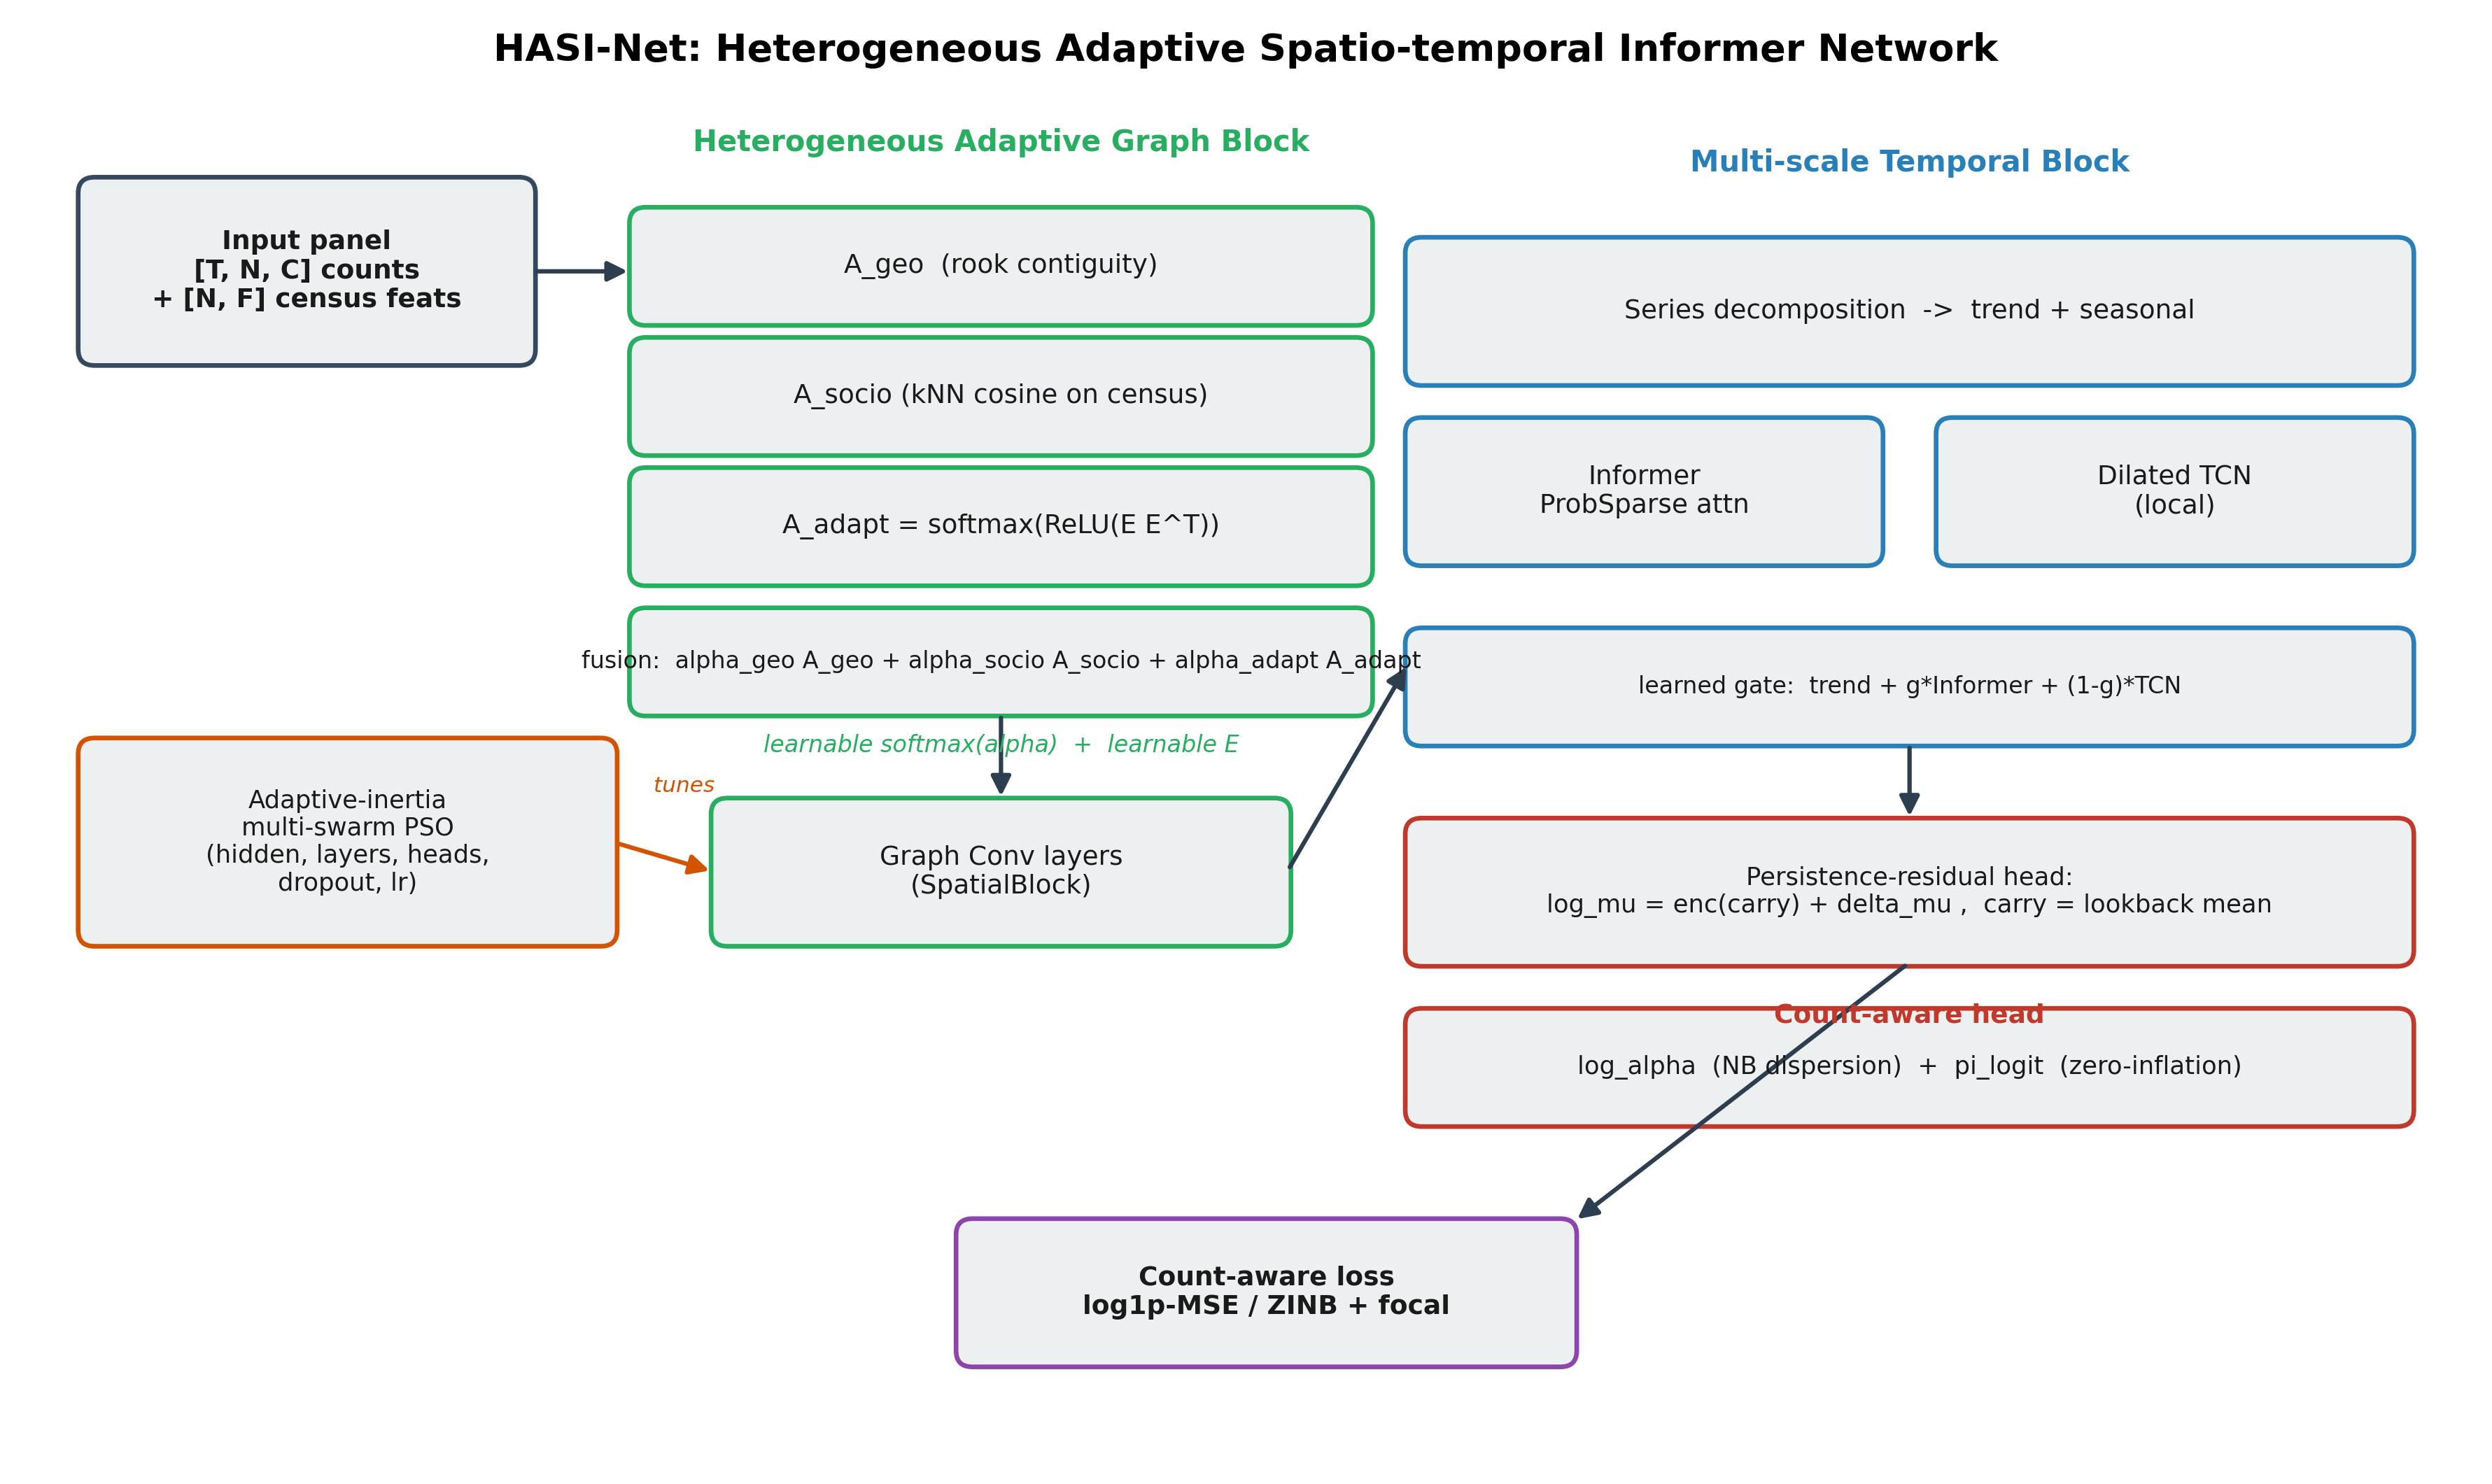
\includegraphics[width=\linewidth]{figures/architecture.png}
\caption{HASI-Net architecture. Input panel $\to$ heterogeneous adaptive graph
block (geographic + socioeconomic + learnable adjacency, softmax-fused) $\to$
multi-scale temporal block (series decomposition, ProbSparse Informer, dilated
TCN, learned gate) $\to$ persistence-residual count-aware head; hyperparameters
selected by adaptive-inertia multi-swarm PSO.}
\label{fig:arch}
\end{figure}

\begin{figure}[t]
\centering
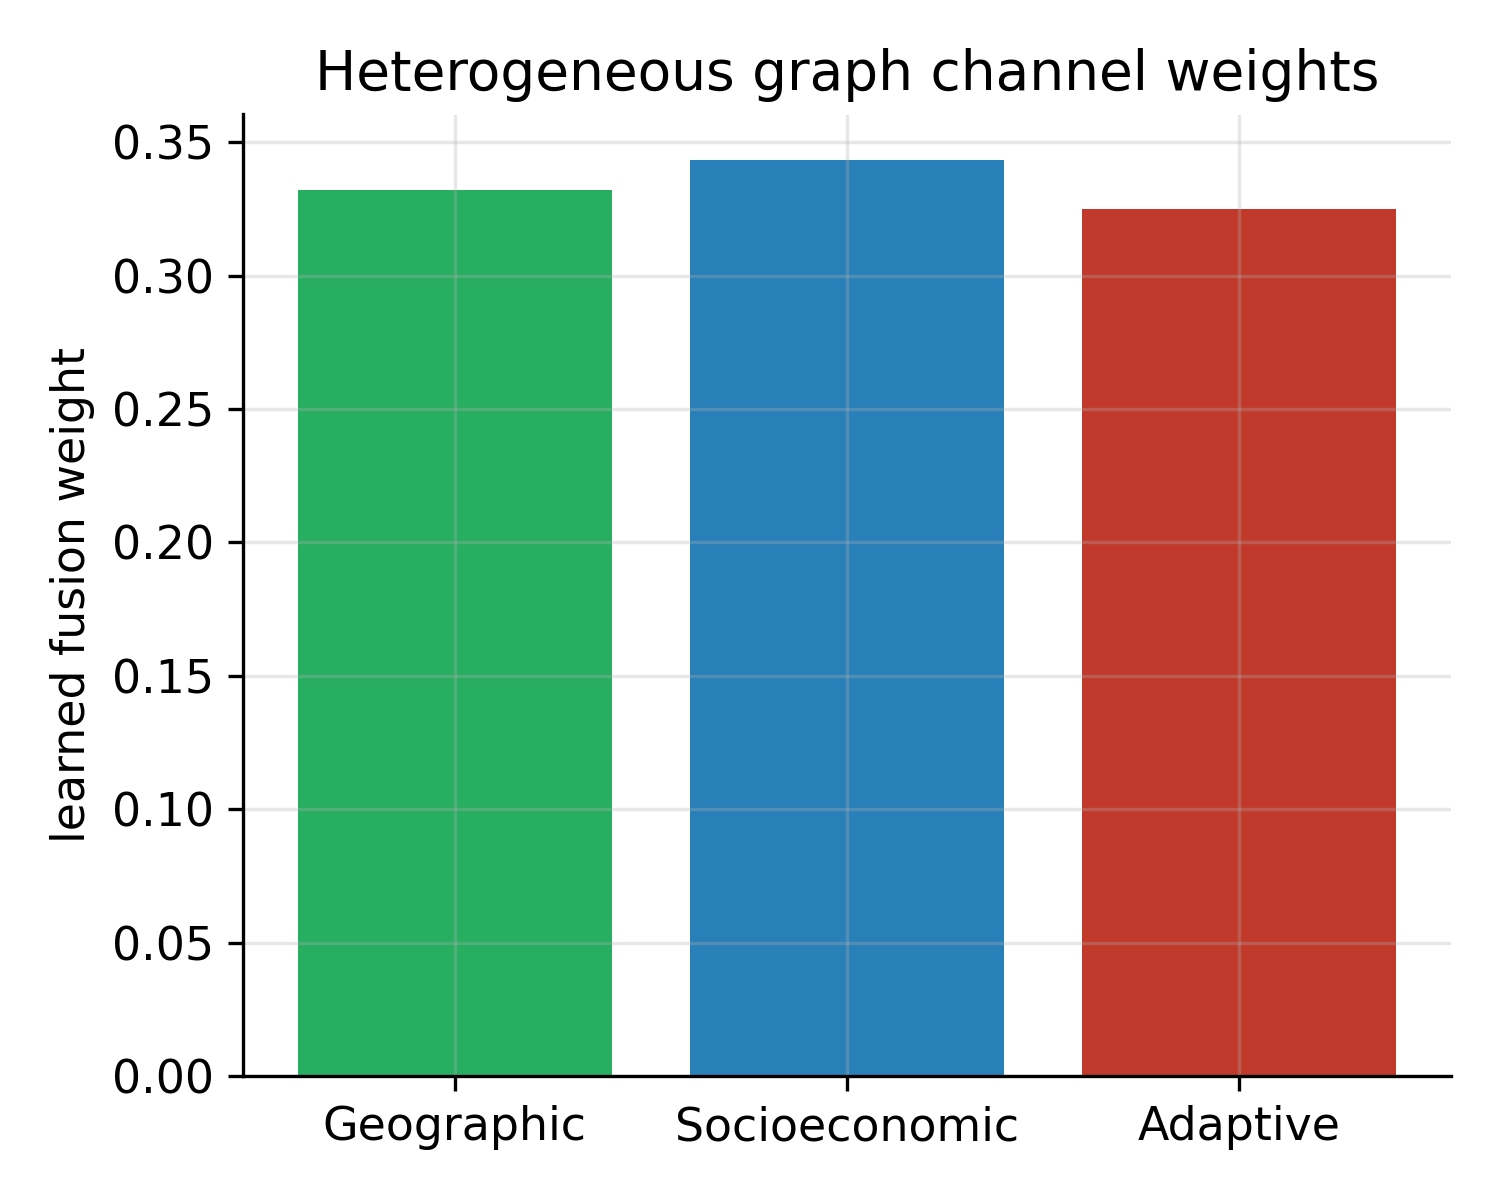
\includegraphics[width=\linewidth]{figures/channel_weights_chicago.png}
\caption{Learned heterogeneous graph channel weights (geographic /
socioeconomic / adaptive) on Chicago---near-balanced ($\approx$0.33 each),
indicating all three notions carry signal on this benchmark.}
\label{fig:channels}
\end{figure}

\begin{figure}[t]
\centering
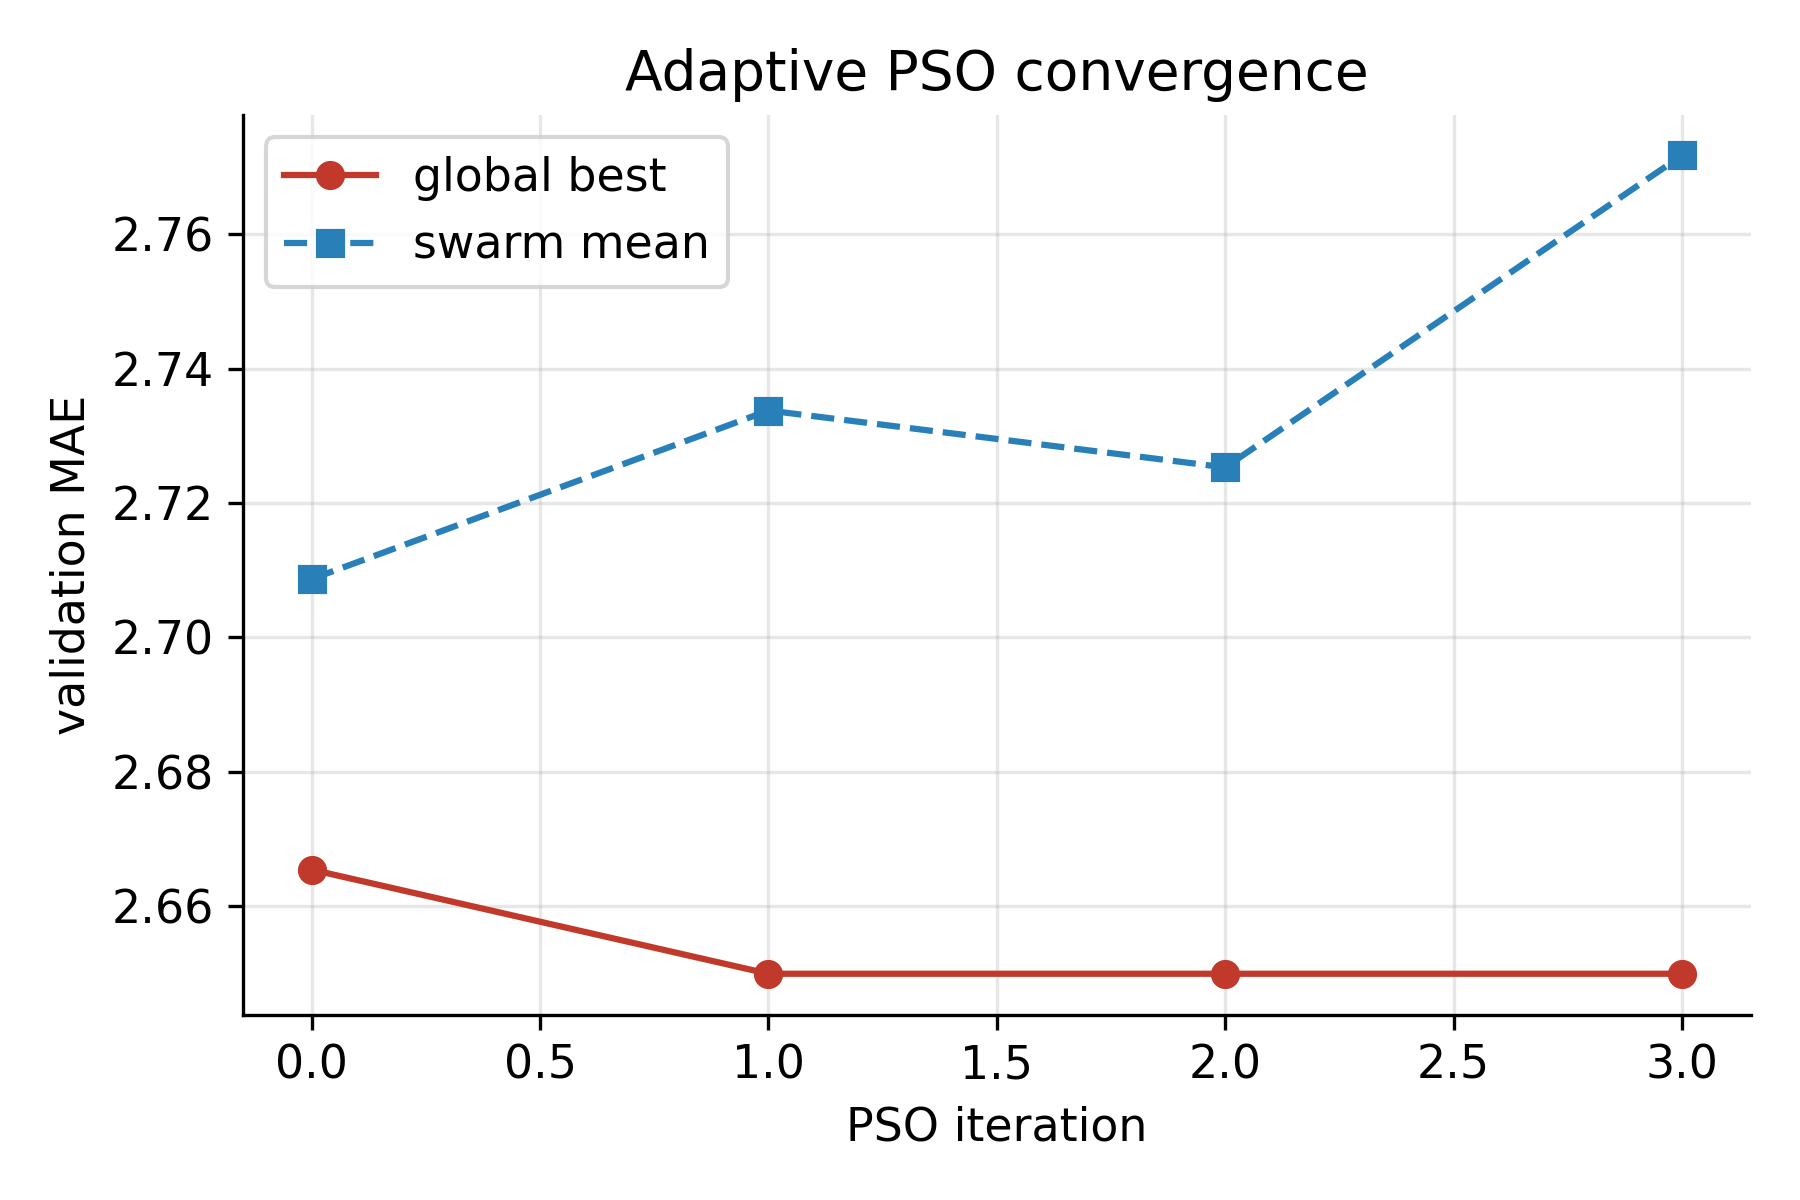
\includegraphics[width=\linewidth]{figures/pso_convergence_chicago.png}
\caption{Multi-swarm PSO convergence on Chicago (seed 42): best and swarm-mean
validation MAE over iterations. Inertia decay broadens early exploration and
sharpens late exploitation; the frozen configuration is reused across all five
seeds.}
\label{fig:pso}
\end{figure}

\begin{figure}[t]
\centering
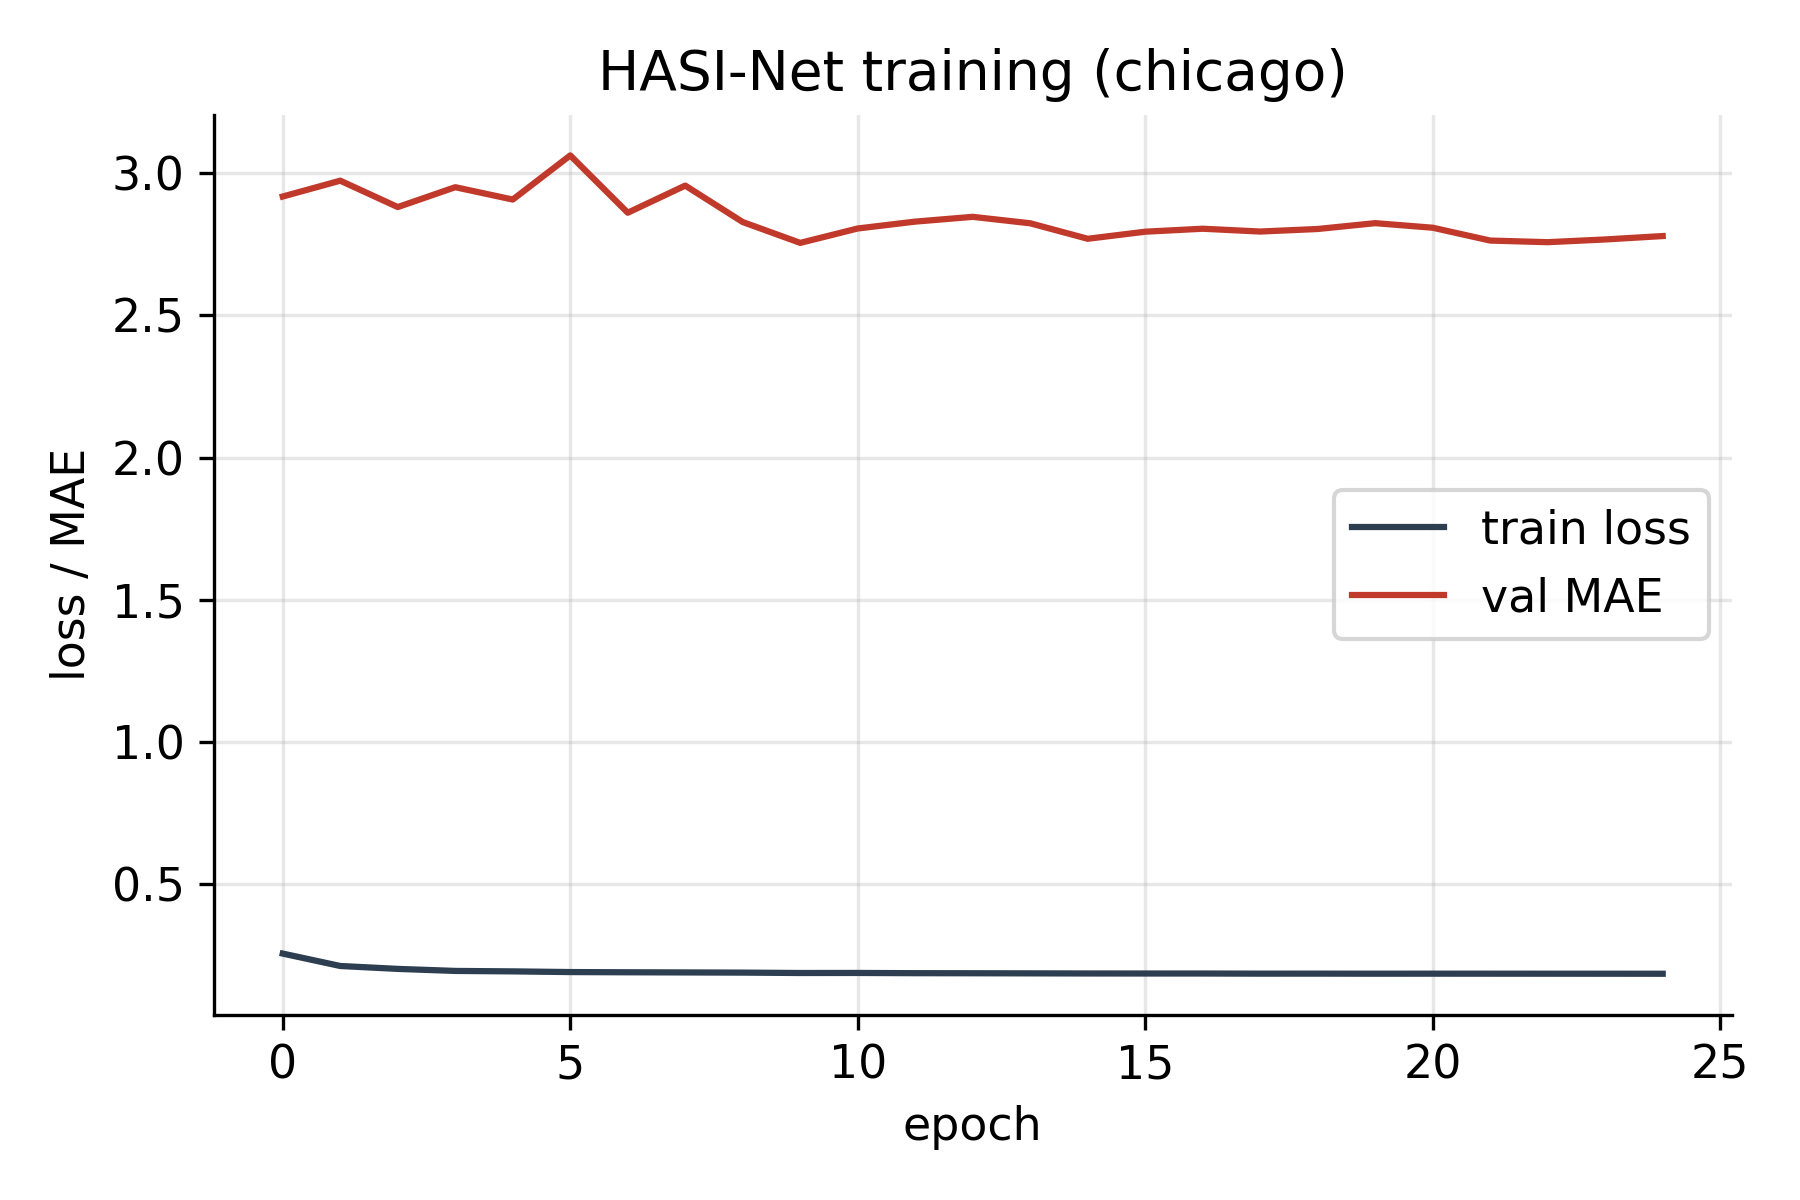
\includegraphics[width=\linewidth]{figures/training_curves_chicago.png}
\caption{Training and validation loss curves for HASI-Net on Chicago across
the five seeds, showing stable convergence and the small-initialised
persistence-residual head keeping the model at the HA carry early in
training.}
\label{fig:training}
\end{figure}

\subsection{Component ablation}\label{sec:ablation}
Table~\ref{tab:ablation} removes one graph channel at a time from the full
model ($H{=}3$, mean$\pm$std over five seeds). Removing any channel degrades
MAE monotonically---Full ($2.633$) $<$ no-adaptive ($2.655$) $<$ no-socio
($2.673$) $<$ no-spatial ($2.686$)---so on this benchmark each of the three
adjacency notions contributes. Reading the degradation magnitudes, removing
the \emph{geographic} channel costs the most ($+0.053$), the socioeconomic
channel next ($+0.040$), and the adaptive channel the least ($+0.022$): the
fixed physical prior is therefore the single largest contributor on Chicago,
which is unsurprising given that the socioeconomic channel operates as a
near-uniform prior here (census features are unavailable for Chicago, so the socio
channel is a near-uniform global-smoothing prior rather than a true
demographic-similarity graph, and is exercised with genuine census features
only on the MP panel), leaving the rook adjacency as the
dominant fixed prior and the learnable channel as a smaller refinement on top
of it. Replacing the log1p-MSE loss with a pure
zero-inflated negative-binomial likelihood (\textit{ZINB-loss}) is the worst
variant ($2.722$): on these small, trended panels a pure count likelihood
pulls the mean off the persistence carry, lowering the likelihood while
raising point MAE and mis-centring the quantiles. This objective mismatch
motivates the companion paper's pivot to a log1p-MSE-plus-pinball
multi-objective loss rather than a pure count likelihood. We report the
ablation as a monotone-degradation result rather than claiming any single
channel dominates: all three carry signal, and the learned fusion weights
(Fig.~\ref{fig:channels}) settle near-balanced ($\approx$0.33 each).

Two further observations sharpen the ablation reading. First, that the
geographic channel is the largest contributor on Chicago is consistent with
the design: with the socioeconomic channel reduced to a near-uniform prior (no
census features for Chicago), the rook adjacency is the dominant fixed prior,
and the learnable adaptive channel acts as a smaller refinement on top of it
rather than displacing it. We expect the ranking to change on the MP panel,
where the socioeconomic channel is genuinely informative---that the relative
contributions are panel-dependent is itself a reason to fuse heterogeneous
priors rather than commit to one. Second, the near-balanced fusion weights
are a \emph{negative} result worth keeping: the optimiser does not collapse
one channel to zero, which means none of the three priors is redundant on this
benchmark, and a designer dropping any one of them a priori would lose signal.
The ZINB-loss degradation is the most decision-relevant finding for the
companion paper: it is the empirical reason we do not use a pure count
likelihood as the production objective, and instead combine log1p-MSE for the
mean with pinball for the quantiles there.

\begin{table}[t]
\centering
\caption{Component ablation on Chicago ($H{=}3$, mean$\pm$std over 5 seeds,
40 epochs). Lower MAE better. Removing any channel degrades MAE.}
\label{tab:ablation}
\begin{tabular}{lr}
\toprule
Variant & MAE\\
\midrule
Full HASI-Net   & \textbf{2.633}$\pm$.019\\
no-adaptive-graph & 2.655$\pm$.022\\
no-socio         & 2.673$\pm$.028\\
no-spatial       & 2.686$\pm$.013\\
ZINB-loss        & 2.722$\pm$.043\\
\bottomrule
\end{tabular}
\end{table}

\subsection{Event verification and hotspot detection}\label{sec:hotspot}
Point MAE rewards getting the level right, which persistence does by carrying
the lookback mean; policing instead acts on \emph{where and when crime spikes}.
Table~\ref{tab:hotspot} reports the event-verification and hotspot metrics
($H{=}3$, mean over five seeds) using the leak-free per-node 90th-percentile
threshold (Sec.~\ref{sec:setup}). The finding extends the persistence result to
the operationally relevant axis: \emph{no model beats persistence by a
practically meaningful margin on event or hotspot metrics either}. GraphWaveNet
is again the marginal, statistically consistent leader (per-node CSI $0.400$
vs HA $0.393$, $p{=}0.003$, 5/5 seeds; MAE $2.552$ vs $2.591$, $p{=}0.008$),
while HASI-Net is mid-pack and marginally \emph{worse} than HA on per-node spike
CSI ($0.383$ vs $0.393$, 0/5 seeds) and on the global high-crime CSI
($0.737$ vs $0.747$, $p{=}0.038$). Friedman's test over the eight models on
per-node CSI rejects equality ($\chi^2{=}27.7$, $p{=}0.0003$), so the ordering
is real, not noise.

Two properties are disclosed rather than hidden. First, \emph{every} model
under-forecasts spike events (frequency bias $0.43$--$0.49{<}1$): deep models
trade a low false-alarm ratio (e.g.\ ST-GCN $0.082$ vs HA $0.130$) for a
slightly lower hit rate, i.e.\ they are more conservative, not more skilful, at
anticipating per-node spikes. Second, the global-pooled threshold (an absolute
high-crime event) gives high CSI for all models ($0.73$--$0.76$) because the
chronically high-crime nodes are persistent and every model reproduces them;
the per-node threshold is the discriminating, operationally meaningful one,
and it is modest for everyone (CSI $\approx0.39$). The top-$k$ hotspot hit rate
(Hit@$5{\approx}0.88$ for nearly all models) is near-saturated for the same
reason---the hotspot node set is persistent---and is not discriminating. The
honest conclusion is that anticipating \emph{transient} per-node spikes is
hard for every method here, persistence included; we argue in the companion
paper that this is precisely the regime where calibrated \emph{conditional}
uncertainty (rather than sharper point forecasts) is the operative need.

\begin{table*}[t]
\centering
\small
\caption{Event verification and hotspot detection, Chicago $H{=}3$ (mean over
5 seeds). Per-node threshold = 90th pct of each node's training counts (leak-free).
POD/FAR/CSI on the per-node spike event; global CSI on the pooled high-crime
event; Hit@5 = top-5 node-set overlap. Best deep model in \textbf{bold}.}
\label{tab:hotspot}
\begin{tabular}{lcccccc}
\toprule
Model & MAE & POD$\uparrow$ & FAR$\downarrow$ & CSI$\uparrow$ & bias & Hit@5\\
\midrule
HA            & 2.591 & 0.417 & 0.130 & 0.393 & 0.479 & 0.879\\
LSTM          & 2.680 & 0.389 & 0.089 & 0.375 & 0.427 & 0.886\\
ST-GCN        & 2.693 & 0.386 & \textbf{0.082} & 0.373 & 0.421 & 0.879\\
GraphWaveNet  & \textbf{2.552} & \textbf{0.426} & 0.132 & \textbf{0.400} & 0.491 & 0.887\\
DCRNN         & 2.680 & 0.391 & 0.092 & 0.376 & 0.431 & 0.879\\
MTGNN         & 2.572 & 0.413 & 0.109 & 0.393 & 0.464 & 0.879\\
InformerOnly  & 2.706 & 0.398 & 0.103 & 0.381 & 0.444 & 0.824\\
HASI-Net      & 2.651 & 0.402 & 0.107 & 0.383 & 0.450 & 0.883\\
\bottomrule
\end{tabular}
\end{table*}

\subsection{Aggregated Madhya Pradesh panel}\label{sec:mp}
The short ($T{=}14$) MP panel is data-limited (only $\approx$9 sliding windows
for $T_w{=}4,H{=}2$), so deep temporal forecasting is fundamentally constrained
there; we use MP primarily for the cross-country transfer and interpretability
analysis of the companion paper rather than headline accuracy. Two structural
points are nevertheless worth recording here. First, the
persistence-residual head keeps HASI-Net at or above the HA baseline rather
than collapsing---the known Transformer failure mode on short series, where an
unconstrained decoder drifts off the carry and underperforms a flat average---so
the architecture degrades \emph{gracefully} in the data-scarce regime rather
than catastrophically, which is the property that makes cross-country transfer
from a data-rich donor (Chicago) worth attempting in the companion paper.
Second, the socioeconomic graph channel, disabled on Chicago for want of
matching census features, is exercised on MP, where Indian Census 2011
district socioeconomics exist; this is the one place in the study where the
heterogeneous graph's second prior contributes, and the ablation cannot isolate
it because the Chicago panel has no socio channel. The applied MP case study,
district risk choropleth, and the disclosed data-scarcity bound on calibration
are the subject of the companion paper; we deliberately do not report a
single-seed MP point-accuracy table here because $T{=}14$ makes any such table
unstable and uninterpretable.

% ===========================================================================
\section{Discussion}\label{sec:disc}
The headline finding is a cautionary one for the field: on a real-geography
monthly crime panel, simple historical-average persistence is a remarkably
strong baseline. It leads raw MAE at every horizon and is matched, not beaten,
by every deep spatio-temporal model---including the more complex HASI-Net---on
both point accuracy and the operationally relevant event-verification and
hotspot metrics. The deep models' edges over persistence, where they exist,
are statistically detectable but practically small (GraphWaveNet $\sim$1.5\%
MAE; HASI-Net best deep model only at the medium horizon). We argue this is
not a failure of architecture but a property of the regime: monthly
community-area crime is highly persistent, so the lookback mean is hard to
beat on the level, and transient per-node spikes are genuinely hard to
anticipate for every method (all models under-forecast spikes, bias${<}1$).
The contribution of this paper is therefore the rigorous, multi-horizon,
multi-seed benchmark with a leak-free event-verification protocol that
\emph{establishes} this finding rather than the usual single-seed table that
overstates a deep model's edge; the heterogeneous-graph methodology and the
ablation showing each adjacency channel contributes; and the narrow but real
result that HASI-Net is the best deep model at the medium horizon and the most
reproducible at the long horizon. The value of the deep approach that
persistence cannot provide---calibrated conditional uncertainty on the
high-crime tail and cross-region transfer---is the subject of the companion
paper, which builds on this strong-persistence finding directly: if point
accuracy is saturated, the deep model must justify itself probabilistically.

\textbf{Relation to the companion paper.} The two papers form a single
argument split for length and readability. This paper establishes the
architecture and the point/event benchmark and reaches the strong-persistence
finding; the companion paper takes that finding as its premise and asks what
the deep model can offer that persistence cannot. Its answer is threefold: a
sparsity-aware calibrated count head (built on the ZINB parametrisation of
Sec.~\ref{sec:head}), a conditional-coverage analysis showing that conformal
baselines catastrophically under-cover the high-crime top decile while the
calibrated head holds it, and a cross-region transfer study
(Chicago$\to$Austin, Chicago$\to$Madhya Pradesh) showing the persistence
carry and the calibrated head transfer across data regimes. The shared
architecture is what makes the transfer principled: the donor and recipient
share the head and the graph block, so transferring weights moves a learned
spatio-temporal representation rather than a brittle city-specific fit.

\textbf{Limitations.} The benchmark is one city at monthly resolution; finer
spatial or temporal granularity, where persistence is weaker, may give the
deep models more room. HASI-Net shows elevated run-to-run MAE variance at the
short horizon, indicating optimization sensitivity worth further work. The
MP panel is annual and very short ($T{=}14$), bounding what any method can
achieve there. ProbSparse attention degenerates to full attention on our short
lookbacks, so its efficiency benefit is not exercised here.

\subsection{Deployment considerations}\label{sec:deploy}
For a policing consumer the operational question is not ``which model has the
lowest MAE'' but ``on which regions and months should we concentrate
resources.'' Two implications follow from the benchmark. First, because
persistence is so strong on the level, a \emph{persistence-first} deployment
(HA as the default forecast, with a deep model consulted only for the
transient-spike signal) is cheap, robust, and hard to beat on the level; we
recommend it as the production baseline against which any deep model must
clearly justify its added cost. Second, the event-verification metrics, not
point MAE, are the deployment-relevant score: a model with marginally lower
MAE but a higher false-alarm ratio (FAR) is worse for an operator whose
credibility depends on not crying wolf. The frequency-bias${<}1$ finding
(every model under-forecasts spikes) means that \emph{no} current model should
be used as a hard spike trigger without a calibration step; this is the
operational motivation for the calibrated probabilistic head of the companion
paper, which converts the under-biased point forecast into a thresholded
mobilisation rule on the upper quantile.

\subsection{Threats to validity}\label{sec:threats}
\textit{Construct validity.} The unified four-category crime space is a
mapping we impose on two heterogeneous registries; while the priority-ordered
rule prevents double-counting, it necessarily loses detail (e.g.\ it merges
several FBI offence codes into ``assault'') and the transfer study inherits
any residual label mismatch. The 90th-percentile per-node threshold defines
``spike'' as a location-relative transient; a different threshold (e.g.\ a
fixed count, or the pooled 90th percentile) would change the POD/FAR/CSI
numbers, which is why we report the pooled threshold alongside for contrast.
\textit{External validity.} The point-accuracy finding is established on one
city at monthly resolution; it should not be generalised to weekly/daily
granularity or to cities with very different reporting geometry without
re-running the benchmark. The MP transfer result (companion paper) is a single
donor--recipient pair and is evidence of \emph{feasibility}, not a general
claim that Chicago-trained weights transfer everywhere.
\textit{Internal validity.} All deep models share the persistence-residual
head, count loss, and evaluation path, which isolates the
spatio-temporal-representation variable but also means the deep models are
not off-the-shelf implementations of the baselines; a reader comparing our
ST-GCN or DCRNN numbers to other papers should note this controlled
configuration. PSO is run once on seed 42 and frozen, so the reported
multi-seed variance understates the variance that would include
hyperparameter-search stochasticity.
\textit{Statistical validity.} Five seeds is modest; we report $p$-values as
ordering diagnostics and do not claim formal significance after
multiple-comparison adjustment. The Friedman tests reject equality of models
at every horizon, but the \emph{practical} effect over HA is small, and we do
not overstate it.
\textit{Scope.} We forecast \emph{reported} crime, not true crime; the
under-reporting caveat in Sec.~\ref{sec:data} bounds any policy reading.

% ===========================================================================
\section{Conclusion}\label{sec:conc}
We presented HASI-Net, a heterogeneous adaptive spatio-temporal Informer
network whose learnable fusion of geographic, socioeconomic and latent
adjacencies, multi-scale temporal block, persistence-residual count-aware
head, and adaptive-inertia PSO together address the coarse, short,
zero-inflated regime of aggregated crime data. Equally, we reported a rigorous
eight-model, five-seed, three-horizon benchmark with a leak-free
event-verification protocol on a real-geography Chicago panel. The honest
finding is that historical-average persistence is a strong baseline that the
deep models match but do not beat on point or event accuracy; HASI-Net is the
best deep model at the medium horizon and the most reproducible at the long
horizon, and each graph channel contributes, but no point-forecast
state-of-the-art claim is warranted. The deep model's defensible value lies in
calibrated conditional uncertainty and cross-region transfer, developed in the
companion paper. All results come from re-runnable CUDA runs with persisted
predictions.

\textit{Practical implication.} For an agency forecasting aggregated regional
crime, the prescription is conservative: deploy persistence as the production
default, measure any deep model against the leak-free event-verification
protocol rather than point MAE, and demand a calibrated upper quantile before
acting on a spike trigger. The deep model's earned place is not in sharper
point forecasts---which persistence already supplies---but in the calibrated
conditional uncertainty and cross-region transfer of the companion paper,
which is where the methodological value of the architecture is realised.

\section*{Reproducibility}
The full pipeline (data download, graph construction, PSO, training,
evaluation, hotspot/event-verification metrics, figures) is released as a
Python package driven by open CUDA notebooks (\texttt{p1\_multiseed\_colab.ipynb},
\texttt{run\_p1\_multiseed.py}, \texttt{run\_p1\_hotspot.py}). Per-seed
predictions are persisted, so every table here is reproducible without
retraining. Re-running the drivers top-to-bottom regenerates every table and
figure in this paper. Specifically: the multi-horizon table
(Table~\ref{tab:multihorizon}) is regenerated by the multi-seed driver over
the five seeds and three horizons; the ablation
(Table~\ref{tab:ablation}) by the same driver with the channel-removal flags;
the event-verification table (Table~\ref{tab:hotspot}) by the hotspot driver
applied to the persisted predictions with the leak-free per-node threshold
(Algorithm~\ref{alg:event}); and the architecture, channel-weight, PSO and
training-curve figures (Figs.~\ref{fig:arch}--\ref{fig:training}) by the
plotting module over the same persisted artifacts. Seeds, splits, and
hyperparameters are fixed in the configuration files so a third party can
reproduce the exact numbers.

\bibliographystyle{IEEEtran}
\bibliography{../references}

\end{document}